\documentclass[12pt]{article}
\usepackage[pdftex]{graphicx}
\pagestyle{plain}
\oddsidemargin  -0.5 cm
\evensidemargin 0.0 cm
\textwidth      6.5in
\headheight     0.0in
\topmargin      -1 cm
\textheight=9.0in

\begin{document}

\section{Neutralinos to Two Leptons}

Focus-point SUSY neutralinos can be studied by looking for events with
missing energy and only two leptons in the final state.  Two
neutralinos, one being the lowest-mass stable particle, $\chi_1^0$,
and the other a heavier neutral combination of winos, binos and
Higgsinos, $\chi_3^0$, are created in the $e^+e^-$ annihilation.  The
$\chi_3^0$ decays into a virtual $Z^0$ and a second $\chi_1^0$, and
both $\chi_1^0$s disappear as missing energy.  We consider here the
case in which the $Z^0$ decays into two leptons ($e^+e^-$ or
$\mu^+\mu^-$).

In addition to Standard Model backgrounds, this mode has significant
SUSY backgrounds, particularly from $\chi_1^+\chi_1^-$ and
$\chi_3^0\chi_2^0$.  We will see later that the Standard Model and
chargino backgrounds can be suppressed by cancelling leptons with
uncorrelated flavors, but the other nutralino mode remains.  The
problem is that this mode has the same $\chi_3^0 \to \ell^+ \ell^-
\chi_1^0$ transition, and the $\chi_2^0$ can decay invisibly into a
$\chi_1^0$ by producing only a $Z^0 \to \nu\bar{\nu}$.  This analysis
can only measure a weighted sum of the $\chi_3^0\chi_1^0$ and
$\chi_3^0\chi_2^0$ cross-sections.

Another measurement, one that is actually aided by the
$\chi_3^0\chi_2^0$ contribution, is the difference in mass between
$\chi_3^0$ and $\chi_1^0$.  Both modes feature a $\chi_3^0 \to
\chi_1^0$ transition; the energy from this transition is shared by the
final-state $\chi_1^0$ and the virtual $Z^0$.  In the limit in which
the $\chi_1^0$ is produced at rest with respect to its parent
$\chi_3^0$, the $Z^0$, and therefore the final-state leptons, carry
all the energy difference.  Hence, the invariant mass spectrum of the
two leptons will have an upper-limit threshold at $m_{\chi_3^0} -
m_{\chi_1^0}$.

\subsection{Standard Model Backgrounds, Event Selection, Polarization}

\begin{figure}[t]
  \begin{center}
    \begin{tabular}{p{0.49\linewidth} p{0.49\linewidth}}
      \begin{center} Unpolarized \end{center} &
      \begin{center} Electrons 95\% Right-Polarized \end{center} \\
      \begin{minipage}{\linewidth} \vspace{-1.2 cm} 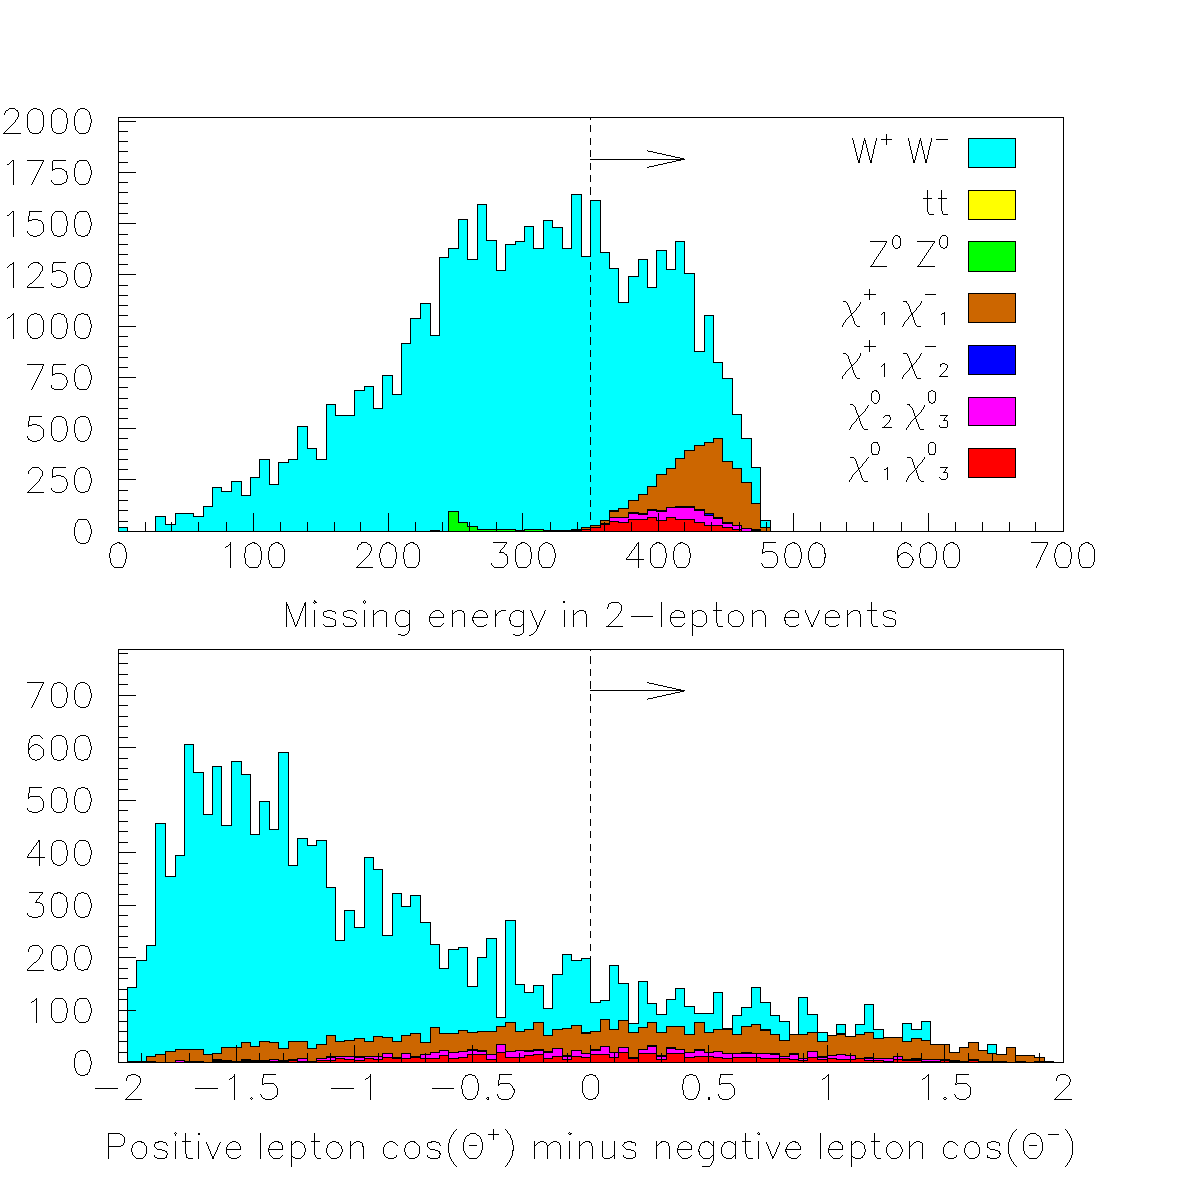
\includegraphics[width=\linewidth]{../pretty_plots/two_leptons_1_fixed.pdf} \end{minipage} &
      \begin{minipage}{\linewidth} \vspace{-1.2 cm} 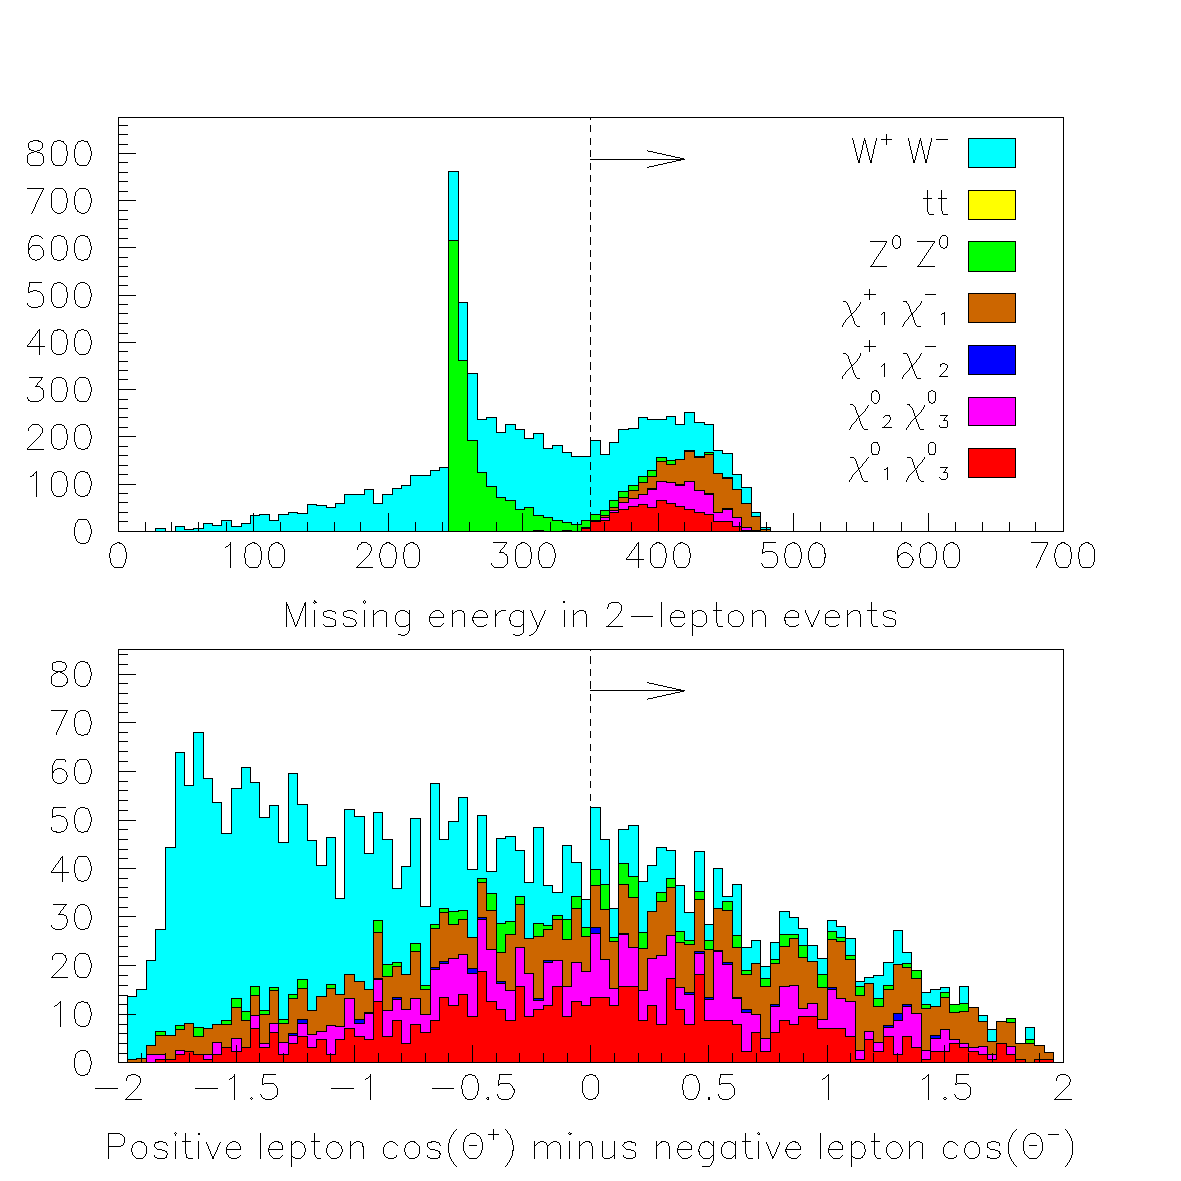
\includegraphics[width=\linewidth]{../pretty_plots/two_leptons_1_fixed_pol.pdf} \end{minipage}
    \end{tabular}


    \caption{Top: Missing energy of all events with two leptons and no
    jets.  Bottom: $\theta$ (or pseudorapidity) correlation of the two
    leptons for all events with more than 350 GeV missing energy.  The
    vertical axes correspond to the expected numbers of events with
    250 fb$^{-1}$.}

    \label{jimpbackgrounds}
  \end{center}
\end{figure}

We considered three potential Standard Model backgrounds: pairs of top
quarks, Z bosons, and W bosons.  Top quark backgrounds are
insignificant to our mode because both sides decay to $W^\pm$ and a
$b$-quark jet, which introduces too many final state charged
particles.  Z bosons are likewise irrelevant because even if one $Z^0$
decays to two tracks and the other decays invisibly, the missing
energy for such an event is always half the beam energy.  That peak
can be avoided on a missing energy plot.  The W-pairs, however, are a
major background, since each $W^\pm$ can decay to a lepton and a
neutrino.  The lepton flavor, electron or muon, is uncorrelated for
W-pairs, but should be the same in our signal.  This fact will be
exploited later.

Only two event selection criteria are used in this analysis: one is
based on missing energy and the other on angular correlations of the
two leptons.  Missing energy is the center-of-mass energy (500 GeV)
minus the energy of all tracks and all unmatched showers.  (Since we
have already restricted ourselves to two visible tracks and no jets,
the missing energy will usually be 500 GeV minus the energy of those
two tracks.)  This missing energy is required to be greater than 350
GeV (shown graphically in the top plots of Figure
\ref{jimpbackgrounds}).

The second requirement takes advantage of the fact that most of the
W-pair production is via a t-channel diagram which correlates the
trajectories of the $W^+$ and $W^-$ with the incident $e^+$ and $e^-$,
respectively.  Taking $\theta^+$ and $\theta^-$ to be the angles
between each final-state lepton and the $e^-$ beam, we want to avoid
the corner of ($\theta^+$, $\theta^-$) in which $\cos\theta^+$ is near
-1 and $\cos\theta^-$ is near 1.  One way to do this is to require
$\cos\theta^+ - \cos\theta^-$ to be greater than some threshold.  We
chose this threshold to be zero (bottom of Figure
\ref{jimpbackgrounds}) because this reduces the W-pair background by a
much-needed factor of ten and because it is a line of symmetry for our
signal.  The shape of the invariant mass distribution is unaffected by
this cut.

Another option for reducing W-pair background is to polarize the
incident beams.  $W^\pm$ couple only to left-handed fermions, so if
the electron beam is right-polarized, the t-channel W-pair production
is turned off, which provides a substantial improvement in
signal-to-background.  In our simulations, the electron beam is taken
to be 95\% right-polarized and the positron beam to be unpolarized.
Plots using polarized beams are displayed on the right-hand sides of
Figures \ref{jimpbackgrounds} and \ref{jimpsubtraction}.

\subsection{SUSY Background and Opposite-Flavor Cancellation}

\begin{figure}[t]
  \begin{center}
    \begin{tabular}{p{0.49\linewidth} p{0.49\linewidth}}
      \begin{center} Unpolarized \end{center} &
      \begin{center} Electrons 95\% Right-Polarized \end{center} \\
      \begin{minipage}{\linewidth} \vspace{-1.2 cm} 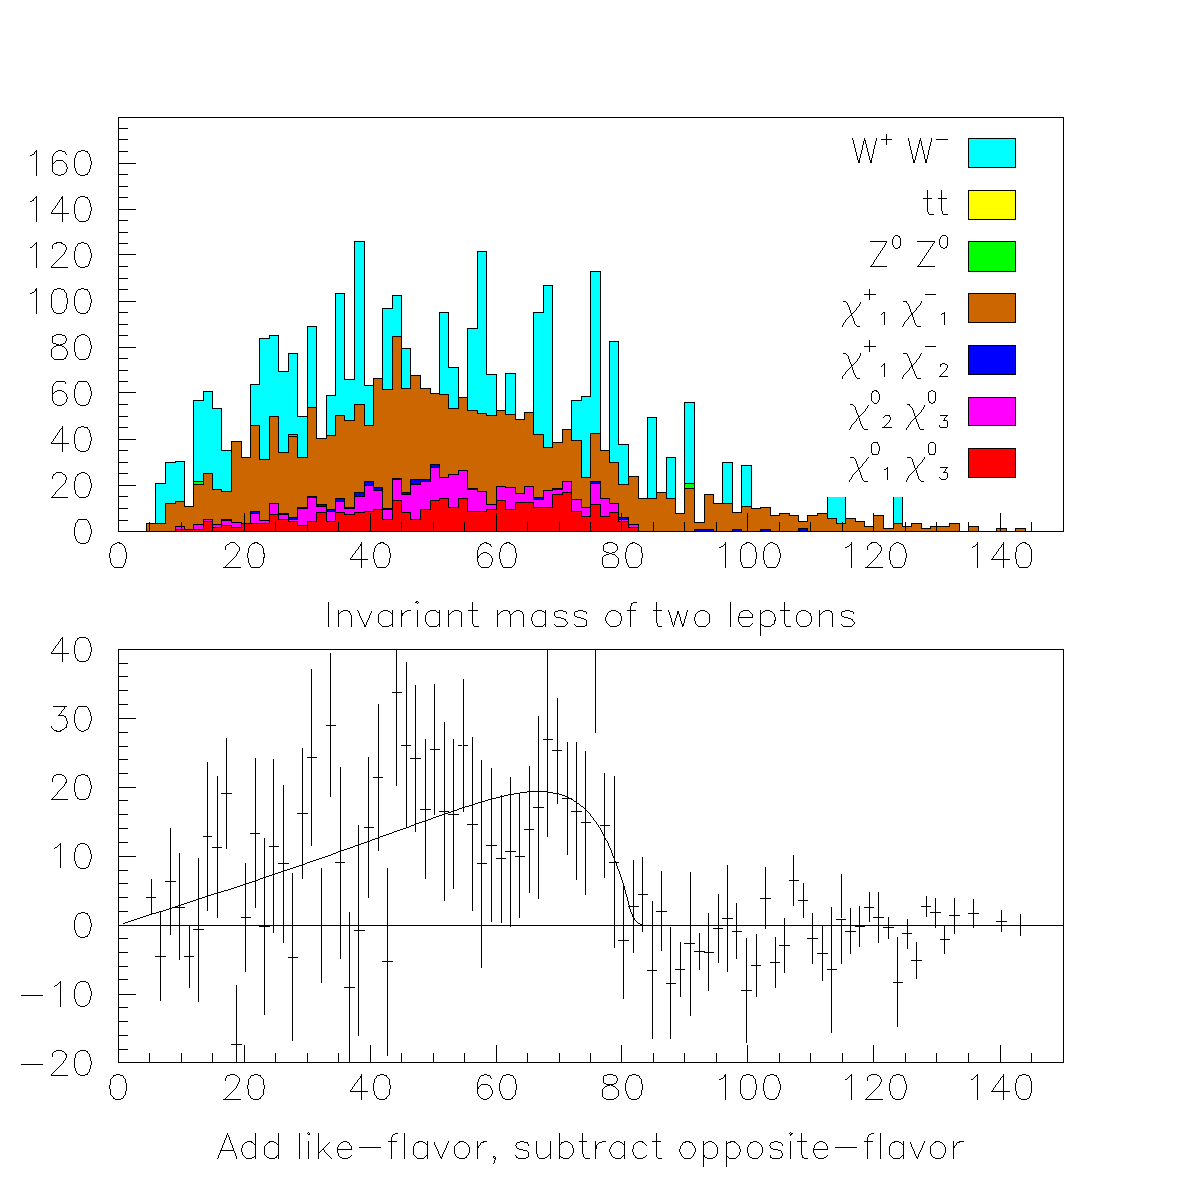
\includegraphics[width=\linewidth]{../pretty_plots/two_leptons_fixed_2.pdf} \end{minipage} &
      \begin{minipage}{\linewidth} \vspace{-1.2 cm} 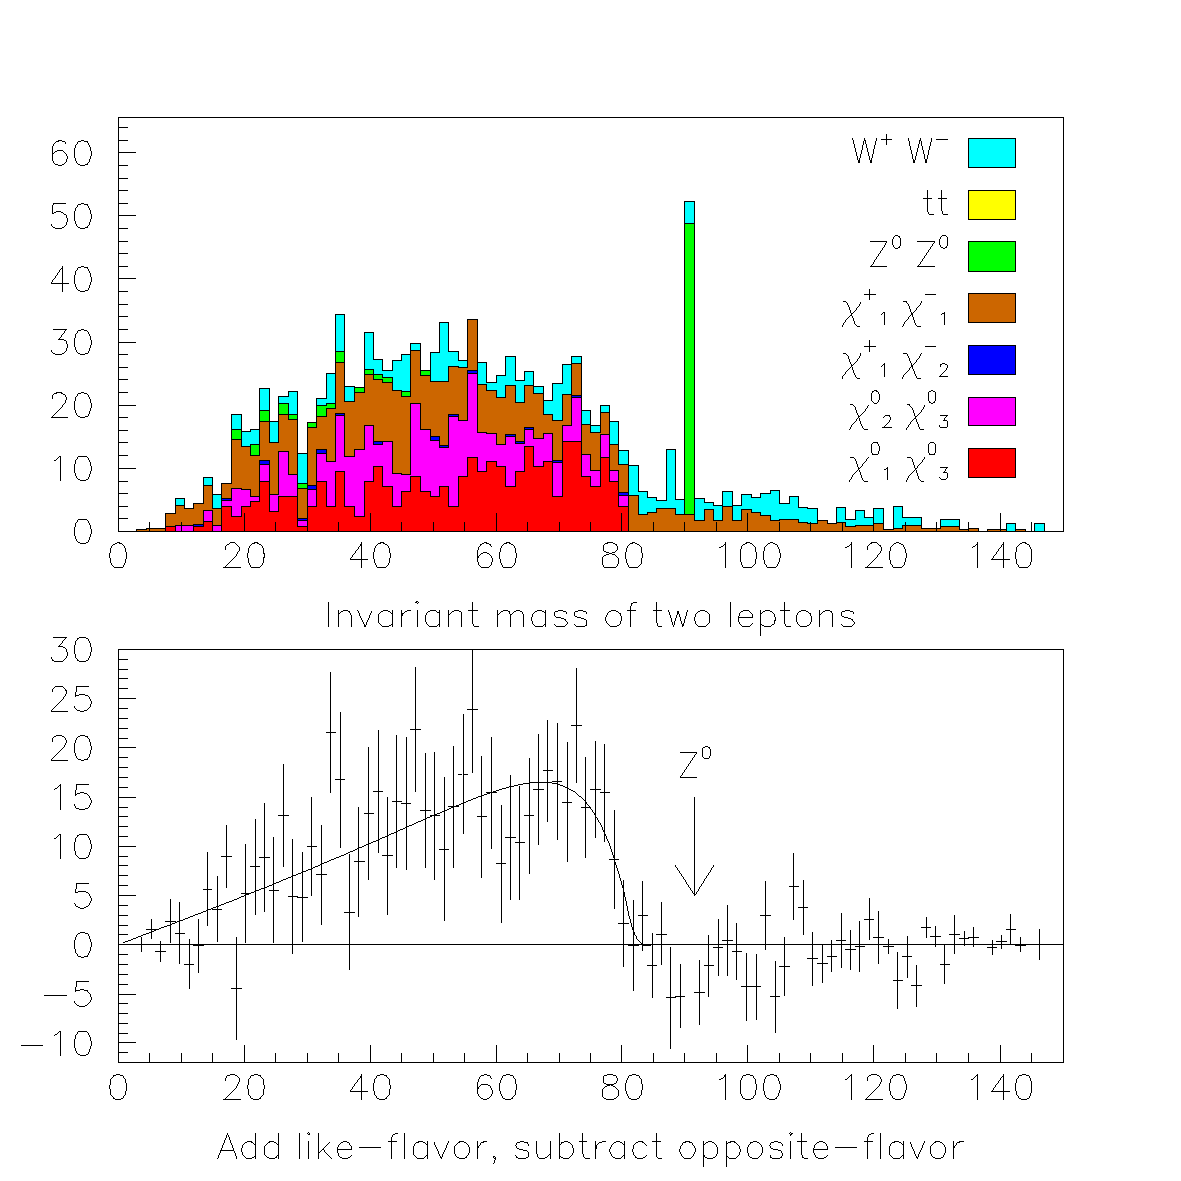
\includegraphics[width=\linewidth]{../pretty_plots/two_leptons_fixed_2_pol.pdf} \end{minipage}
    \end{tabular}

    \caption{Top: Invariant mass distribution of all contributions.
    The red and purple distributions are the signals
    $\chi_3^0\chi_1^0$ and $\chi_3^0\chi_2^0$; the cyan and brown are
    Standard Model W-pairs and SUSY $\chi_1^+\chi_1^-$.  Bottom:
    Invariant mass distribution where $e^+e^-$ and $\mu^+\mu^-$ events
    were given a weight of 1 and $e^\pm\mu^\mp$ and $\mu^\pm e^\mp$
    events were given a weight of -1.  In the polarized sample, we
    suppressed the bin containing real $Z^0$ decays.  The vertical
    axes and error bars correspond to the expected numbers of events
    with 250 fb$^{-1}$.}

    \label{jimpsubtraction}
  \end{center}
\end{figure}

Even after the selection criteria described in the last section,
W-pairs are still a significant background in the unpolarized sample.
In addition, $\chi_1^+\chi_1^- \to$ two leptons contributes at an even
larger scale, as shown in the top plots of Figure
\ref{jimpsubtraction}.  Each $\chi_1^\pm$ can decay to a $W^\pm$, and
$\chi_1^+\chi_1^-$ events typically have more missing energy than
$W^+W^-$.

Fortunately, the two leptons from W-pairs and from $\chi_1^+\chi_1^-$
both come from independent $W^\pm$ decays, and therefore have
uncorrelated flavors (electron or muon).  In the signal modes,
$\chi_3^0\chi_1^0$ and $\chi_3^0\chi_2^0$, the lepton pair comes from
a single $Z^0$ decay, so it should be either $e^+e^-$ or $\mu^+\mu^-$.
If events with same-flavor leptons are added to a histogram (filled
with weight 1) and events with opposite-flavor leptons are subtracted
(filled with weight -1), both backgrounds will cancel in the average
and the signal will add constructively.  We used this technique to
subtract the remaining backgrounds, yielding the difference in the
bottom plots of Figure \ref{jimpsubtraction}.  We assumed an
integrated luminosity of 250 fb$^{-1}$ for each of the two samples,
polarized and unpolarized.

With right-handed electrons, the W-pair background is eliminated and
the $\chi_1^+\chi_1^-$ background is significantly reduced.  Z-pairs
in the polarized sample, however, contribute more to the two-lepton
mode (even though the overall cross-section is lower) as seen in the
top of Figure \ref{jimpbackgrounds}.  Most of these Z-pairs are
eliminated with the missing energy cut, but if the missing energy is
overestimated by 100 GeV, a few events can leak into the invariant
mass plot.  This is easily handled, though, because a pair of leptons
from a single real $Z^0$ decay will have an invariant mass at the
$Z^0$ mass, and this bin can be excluded from the fit.

Some care must be taken in interpreting these plots because they
represent the case of ideal lepton flavor tagging.  If flavor tagging
efficiency is only 90\%, the signal mound would be reduced in height
by a factor of 0.9.  Worse yet, if the tagging algorithm favored one
flavor over the other, the backgrounds wouldn't exactly cancel, and
would distort the shape of the threshold.  That said, a realistic
detector should have little difficulty distinguishing between
$\sim$100 GeV electron showers and minimum-ionizing muon showers,
particularly if the muon identification is aided by a muon detector
beyond the calorimeters.

\subsection{Cross-section Constraints}

\begin{table}
  \begin{center}
    \begin{tabular}{c p{6 cm} p{6 cm}}
      & \begin{center} Unpolarized \end{center} &
      \begin{center} Electrons 95\% Right-Polarized \end{center} \\
      $\chi_3^0\chi_1^0$ &
      \begin{center} \begin{minipage}{2.3 cm} \vspace{-1 cm} \begin{center} \begin{tabular}{r c l} $\mathcal{B}\varepsilon$ &=& 3.33\% \\
      $\sigma$ &=& 50.5 fb \end{tabular} \end{center} \end{minipage} \end{center} &
      \begin{center} \begin{minipage}{2.3 cm} \vspace{-1 cm} \begin{center} \begin{tabular}{r c l} $\mathcal{B}\varepsilon$ &=& 2.86\% \\
      $\sigma$ &=& 44.1 fb \end{tabular} \end{center} \end{minipage} \end{center} \\
      $\chi_3^0\chi_2^0$ &
      \begin{center} \begin{minipage}{2.3 cm} \vspace{-1 cm} \begin{center} \begin{tabular}{r c l} $\mathcal{B}\varepsilon$ &=& 1.36\% \\
      $\sigma$ &=& 81.6 fb \end{tabular} \end{center} \end{minipage} \end{center} &
      \begin{center} \begin{minipage}{2.3 cm} \vspace{-1 cm} \begin{center} \begin{tabular}{r c l} $\mathcal{B}\varepsilon$ &=& 1.35\% \\
      $\sigma$ &=& 70.9 fb \end{tabular} \end{center} \end{minipage} \end{center} \\
      Events seen & \begin{center} \vspace{-0.8 cm} 605 $\pm$ 75 \end{center} &
      \begin{center} \vspace{-0.8 cm} 528 $\pm$ 38 \end{center}
    \end{tabular}

    \caption{Branching fractions times efficiencies
    $\mathcal{B}\varepsilon$ (the number seen in the invariant mass
    plot divided by the number generated in Monte Carlo) and
    cross-sections $\sigma$ for each of the two signal modes, and the
    number of events seen in the invariant mass plot, where the two
    modes can't be separated.  The uncertainty in the number of events
    seen assumes 250 fb$^{-1}$ in each sample.}
    \label{crosssections}
  \end{center}
\end{table}

As explained above, we can only measure a weighted sum of the
cross-sections of $\chi_3^0\chi_1^0$ and $\chi_3^0\chi_2^0$.  The
weighting factors depend on the branching fractions of
$\chi_3^0\chi_1^0$ and $\chi_3^0\chi_2^0$ to two leptons and on the
efficiencies of these modes through our event selection.  The event
selection efficiencies alone are nearly 50\% in all cases, due almost
entirely to the angular cut.  The branching fractions depend on
well-known $Z^0$ branching ratios and the branching fraction of heavy
neutralinos to $Z^0 \chi_1^0$, which is 100\%.  Therefore, we combine
all branching fractions and efficiencies into a single factor
$\mathcal{B}\varepsilon$ with no uncertainties.  The
$\mathcal{B}\varepsilon$ factors and cross-sections can be found in
Table \ref{crosssections}, along with the number of events seen in the
invariant mass plot, which is the source of uncertainty in this
analysis.

The number of events seen is derived from the branching fractions,
efficiencies, and cross-sections like this:
\begin{equation}
  (\sigma \mathcal{B}\varepsilon)_{\chi_3^0\chi_1^0} +
  (\sigma \mathcal{B}\varepsilon)_{\chi_3^0\chi_2^0} =
  \frac{\mbox{events seen}}{\mbox{integrated luminosity}}
\end{equation}
where the integrated luminosity is 250 fb$^{-1}$.  Inserting our
results, we obtain two constraints on $\sigma_{\chi_3^0\chi_1^0}$ and
$\sigma_{\chi_3^0\chi_2^0}$.
\begin{eqnarray}
  (0.0138 \mbox{ fb}^{-1}) \, \sigma_{\chi_3^0\chi_1^0} \mbox{\hspace{0.6 cm}} +
  & (0.00562 \mbox{ fb}^{-1}) \, \sigma_{\chi_3^0\chi_2^0} &= \mbox{\hspace{0.2 cm}} 1 \pm 0.12 \\
  (0.0135 \mbox{ fb}^{-1}) \, \sigma_{\chi_3^0\chi_1^0\mbox{\scriptsize, pol}} \mbox{\hspace{0.6 cm}} +
  & (0.00639 \mbox{ fb}^{-1}) \, \sigma_{\chi_3^0\chi_2^0\mbox{\scriptsize, pol}} &= \mbox{\hspace{0.2 cm}} 1 \pm 0.072
\end{eqnarray}
These constraints are, of course, consistent with the generated
cross-sections.

\subsection{Mass Difference Constraints}

Using the three-body fit function described elsewhere, we fit each of
our invariant mass distributions for the upper edge of the
distribution.  Two parameters were floated in the fit: overall
normalization and the mass difference $m_{\chi_3^0} - m_{\chi_1^0}$.
The errors obtained from this fit are
\begin{eqnarray}
  & & \pm \, 2.3 \mbox{ GeV for the unpolarized sample and} \\
  & & \pm \, 0.72 \mbox{ GeV for the polarized sample.}
\end{eqnarray}
These uncertainties are to be understood as approximate, as some
improvement in the fit method will be needed for the full analysis.
If the data is simply binned into a histogram for background
subtraction by the above method, the fitted value of the threshold
varies with the bin spacing.  The uncertainty does not vary, however,
and an unbinned maximum likelihood fit of the unpolarized sample
aggreed approximately with the 2.3 GeV uncertainty quoted above,
although even that was difficult to interpret because the maximum of
the log likelihood is not a smooth function.  (It is difficult to
introduce background subtraction into the likelihood, since the
probability distribution is zero above the threshold.)

Though a great deal of care will need to be taken to fit the threshold
properly, unbiased by bin effects and including the much-needed
background subtraction, a few-GeV statistical error on the 83 GeV mass
difference should be attainable.

%% unpol

%%  Convergence when estimated distance to minimum (EDM) .LT.  0.10E+01

%%  FCN=   78.68930     FROM MINOS     STATUS=SUCCESSFUL    94 CALLS      157 TOTAL
%%                      EDM=  0.67E-03    STRATEGY= 1      ERROR MATRIX ACCURATE 

%%   EXT PARAMETER                  PARABOLIC         MINOS ERRORS        
%%   NO.   NAME        VALUE          ERROR      NEGATIVE      POSITIVE   
%%    1      P1        3.3626       0.91919       -1.0689       0.99833    
%%    2      P2        82.809        1.7829       -1.9301        2.3364    

%%  CHISQUARE = 0.9045E+00  NPFIT =    89



%% polarized

%%  FCN=   78.64595     FROM MINOS     STATUS=SUCCESSFUL    54 CALLS      122 TOTAL
%%                      EDM=  0.16E-04    STRATEGY= 1      ERROR MATRIX ACCURATE 

%%   EXT PARAMETER                  PARABOLIC         MINOS ERRORS        
%%   NO.   NAME        VALUE          ERROR      NEGATIVE      POSITIVE   
%%    1      P1        5.0174       0.53073      -0.51458       0.53905    
%%    2      P2        82.526       0.71509      -0.72388       0.70643    

%%  CHISQUARE = 0.8642E+00  NPFIT =    93


\end{document}







%% two-jets unpol

%%  FCN=   46.52510     FROM MINOS     STATUS=PROBLEMS    1006 CALLS     1088 TOTAL
%%                      EDM=  0.95E-02    STRATEGY= 1      ERROR MATRIX ACCURATE 

%%   EXT PARAMETER                  PARABOLIC         MINOS ERRORS        
%%   NO.   NAME        VALUE          ERROR      NEGATIVE      POSITIVE   
%%    1      P1        5.6505       0.97403       -1.1361        1.0325    
%%    2      P2        78.181       0.98434                      1.2990    
%%    3      P3        3.3971        1.5376       -1.2710        1.4146    
%%    4      P4        55.255        1.6190       -4.1151        1.9801    

%%  CHISQUARE = 0.9495E+00  NPFIT =    53

%% electrons right-polarized

%%  FCN=   59.14009     FROM MINOS     STATUS=SUCCESSFUL   732 CALLS      807 TOTAL
%%                      EDM=  0.24E-02    STRATEGY= 1      ERROR MATRIX ACCURATE 

%%   EXT PARAMETER                  PARABOLIC         MINOS ERRORS        
%%   NO.   NAME        VALUE          ERROR      NEGATIVE      POSITIVE   
%%    1      P1        44.517        2.1590       -1.8755        2.2826    
%%    2      P2        81.393       0.26156      -0.28140       0.22159    
%%    3      P3        22.553        3.5912       -3.5976        3.3846    
%%    4      P4        58.492       0.67531      -0.47757       0.66081    

%%  CHISQUARE = 0.9539E+00  NPFIT =    66






%% two-jets nobump unpol

%%  FCN=   15.38906     FROM MINOS     STATUS=SUCCESSFUL    96 CALLS      153 TOTAL
%%                      EDM=  0.60E-03    STRATEGY= 1      ERROR MATRIX ACCURATE 

%%   EXT PARAMETER                  PARABOLIC         MINOS ERRORS        
%%   NO.   NAME        VALUE          ERROR      NEGATIVE      POSITIVE   
%%    1      P1        5.8900       0.97118      -0.90616        1.1962    
%%    2      P2        79.356       0.80749      -0.99223       0.81264    

%%  CHISQUARE = 0.6995E+00  NPFIT =    24

